\documentclass[MASTER.tex]{subfiles}
\begin{document}
\begin{frame}
\frametitle{The \texttt{numpy} package}
\Large
\begin{itemize}
\item The Python programming language was not initially designed for numerical computing, but attracted the attention of the scientific/engineering community early on.

\item NumPy is an extension to the Python programming language, adding support for large, multi-dimensional arrays and matrices, along with a large library of high-level mathematical functions to operate on these arrays. 
\end{itemize}
\end{frame}
%====================================================%
\begin{frame}
\begin{itemize}
\item The ancestor of NumPy, Numeric, was originally created by Jim Hugunin with contributions from several other developers. 
\item In 2005, Travis Oliphant created NumPy by incorporating features of Numarray into Numeric with extensive modifications. 
\end{itemize}

\end{frame}
%====================================================%
\begin{frame}
\frametitle{The \texttt{numpy} package}
\Large	
	
\begin{itemize}
\item NumPy is open source and has many contributors.
\item \textbf{Website} http://www.numpy.org/
\end{itemize}

\end{frame}

%====================================================%
\begin{frame}
\frametitle{The \texttt{numpy} package}
\Large	
\textbf{Useful Commands for simulation exercises}
\begin{itemize}
\item \texttt{random.randint(a, b)} - Return a random integer N such that $a \leq N \leq b$.

\item \texttt{random.choice(seq)} - return a random element from the non-empty sequence \texttt{seq}. \\ If \texttt{seq} is empty, raises \texttt{IndexError}.

\item \texttt{random.sample(population, k)} - 
Return a k length list of unique elements chosen from the population sequence. Used for random \textit{sampling without replacement}.
\end{itemize}
\end{frame}
%=========================================== %
\begin{frame}
	\begin{figure}
\centering
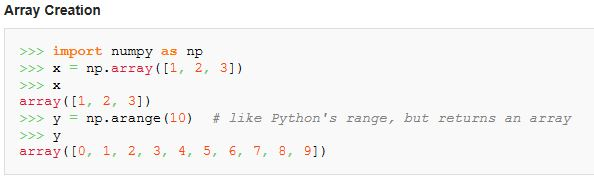
\includegraphics[width=1.16\linewidth]{numpyarraycreation}

\end{figure}

\end{frame}	
%========================================== %
\begin{frame}
	\begin{figure}
		\centering
		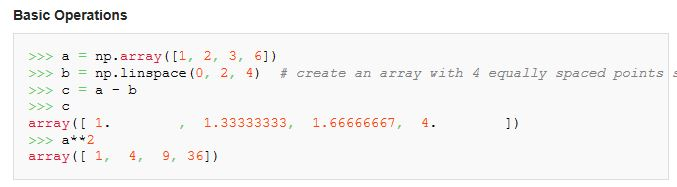
\includegraphics[width=1.15\linewidth]{numpybasicoperations}

	\end{figure}
	
\end{frame}	
%========================================== %
\end{document}